% SOF
% LaTeX macro to try fill up a Sudoku case with numbers which may be right,

% TODO: try to add this to an existing sudoku package.

\documentclass{article}

\usepackage{tikz}
\usepackage{listofitems}
%\usetikzlibrary{arrows}

% Fill a Sudoku case with potential numbers.
\newcommand{\sudokucase}[3]{(#1,#2)::\readlist\valeurs{#3}
\readlist\cx{0.2,0.5,0.8,0.2,0.5,0.8,0.2,0.5,0.8}
\readlist\cy{0.8,0.8,0.8,0.5,0.5,0.5,0.2,0.2,0.2}
\ifnum\valeurslen=1 \node at (#1-0.5,9.5-#2){\huge\textsc{#3}};\else
\foreachitem\valeur\in\valeurs{\node at (#1-1+\cx[\valeur],9-#2+\cy[\valeur]) {\footnotesize{\textit{\valeur}}};}
\fi}

\begin{document}
% Usage
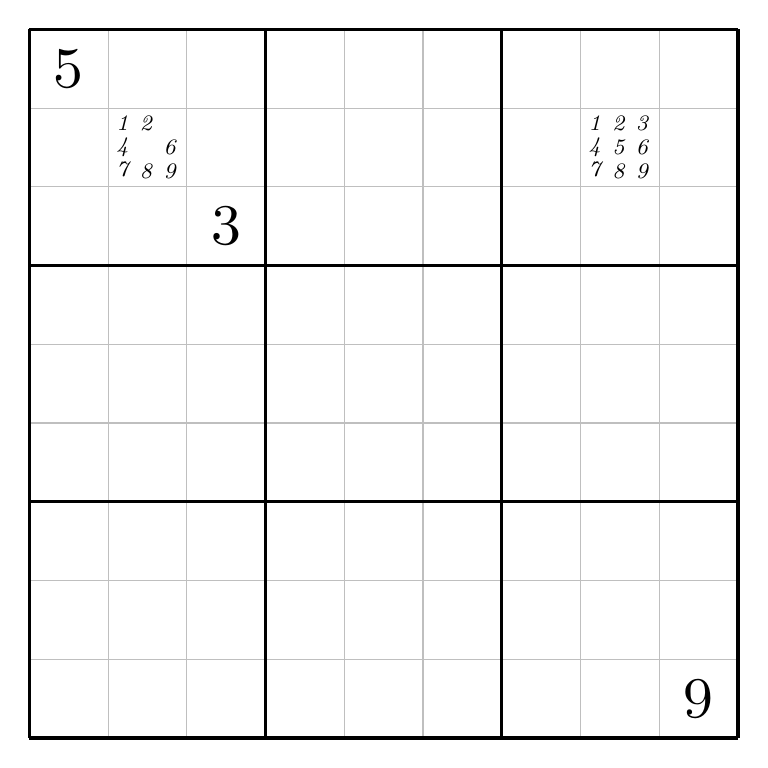
\begin{tikzpicture}[scale=1]
\draw[help lines, thin, lightgray](0,0) grid(9,9);
\draw[help lines, very thick, black, step=3](0,0) grid(9,9);
\sudokucase{1}{1}{5};
\sudokucase{2}{2}{1,2,4,6,7,8,9};
\sudokucase{8}{2}{1,2,3,4,5,6,7,8,9};
\sudokucase{3}{3}{3};
\sudokucase{9}{9}{9};
\end{tikzpicture}

\end{document}
% EOD

% EOF
